% -*- coding: utf-8 -*-

\chapter{Transformaciones relativas}\label{ap:transformaciones}

La transformación relativa entre el sistema de referencia $i$ y el sistema de referencia $j$ viene dado por
\begin{equation}\label{eq:ij}
\vec{x_{ij}} = [x_{ij} y_{ij} \theta_{ij}]^{T}
\end{equation}

El operador composición $\oplus$ entre dos transformaciones relativas se define como:
\begin{equation}\label{eq:composicion}
    \vec{x_{ik}} = \vec{x_{ij}} \oplus \vec{x_{jk}} = \pmatrix{x_{ij} + x_{jk}cos \theta_{ij} - y_{jk}sin \theta_{ij}\cr y_{ij} + x_{jk}sin \theta_{ij} + y_{jk}cos \theta{ij}\cr \theta_{ij} + \theta_{jk}}
\end{equation}

\begin{figure}[h]
  % Requires \usepackage{graphicx}
  \centering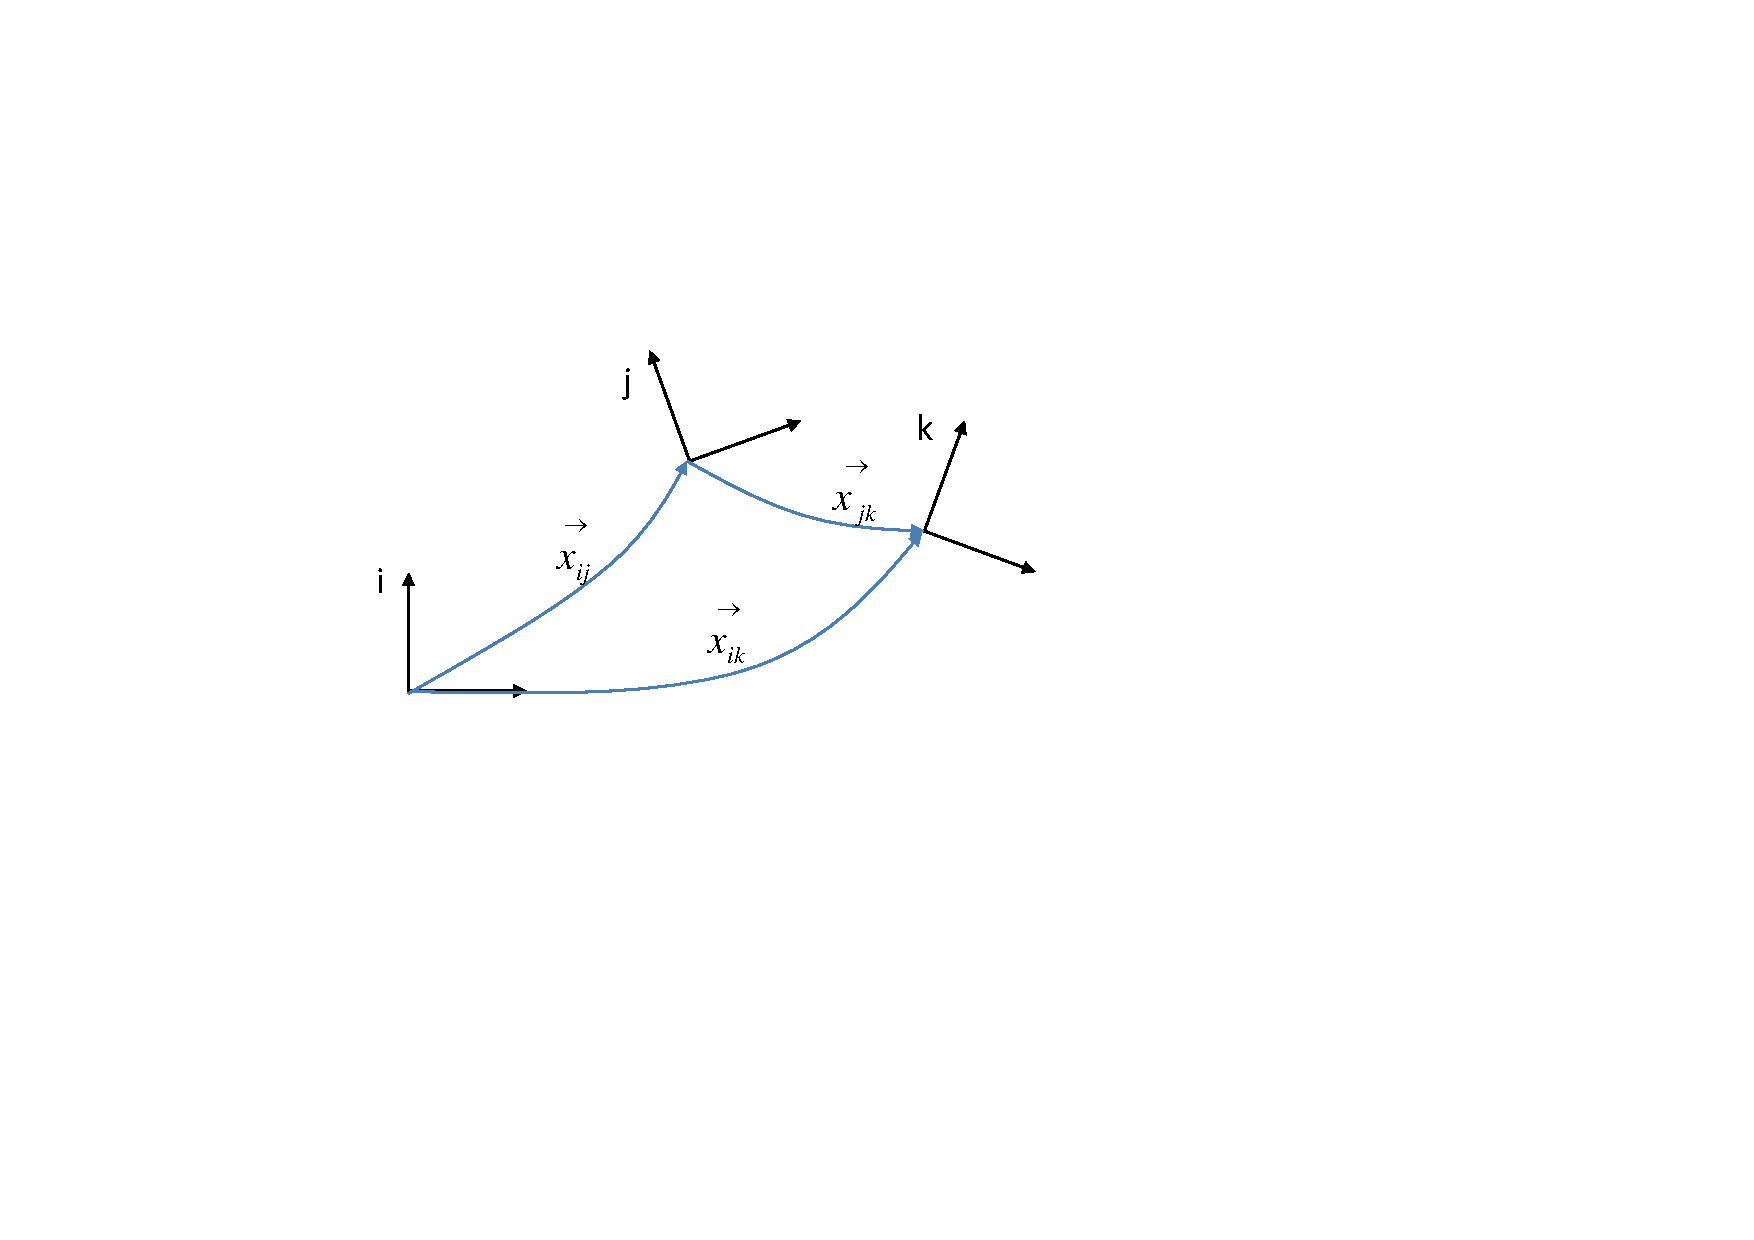
\includegraphics[width=0.5\textwidth]{comp}\\
  \caption{Composición de transformaciones relativas}\label{fg:comp}
\end{figure}

Si se calcula su jacobiana respecto de la primera transformación se obtiene:
\begin{equation}\label{eq:J1}
    F1(x_{ij},x_{jk}) = \frac{\delta x_{ik}}{\delta x_{ij}} = \left(
  \begin{array}{ccc}
    1 & 0 & -x_{jk}sin \theta_{ij}-y_{jk}cos \theta_{ij} \\
    0 & 1 & x_{jk}cos \theta_{ij}-y_{jk}sin \theta{ij} \\
    0 & 0 & 1 \\
  \end{array}
\right)
\end{equation}

La jacobiana respecto a la segunda transformación será:

\begin{equation}\label{eq:J2}
    F2(x_{ij},x_{jk}) = \frac{\delta x_{ik}}{\delta x_{jk}} = \left(
  \begin{array}{ccc}
    cos \theta_{ij} & -sin \theta_{ij} & 0 \\
    sin \theta_{ij} & cos \theta_{ij} &  0\\
    0 & 0 & 1 \\
  \end{array}
\right)
\end{equation}

El operador inversión $\ominus$ de la transformación relativa entre el sistema de coordenadas $i$ y el sistema de coordenadas $j$ se define como:

\begin{equation}\label{eq:inversion}
    \vec{x_{ji}} = \ominus \vec{x_{ij}} = \pmatrix{-x_{ij}cos \theta_{ij}-y_{ij}sin \theta_{ij}\cr x_{ij}sin \theta_{ij} - y_{ij}cos \theta_{ij}\cr - \theta_{ij}}
\end{equation}

\begin{figure}[h]
  % Requires \usepackage{graphicx}
  \centering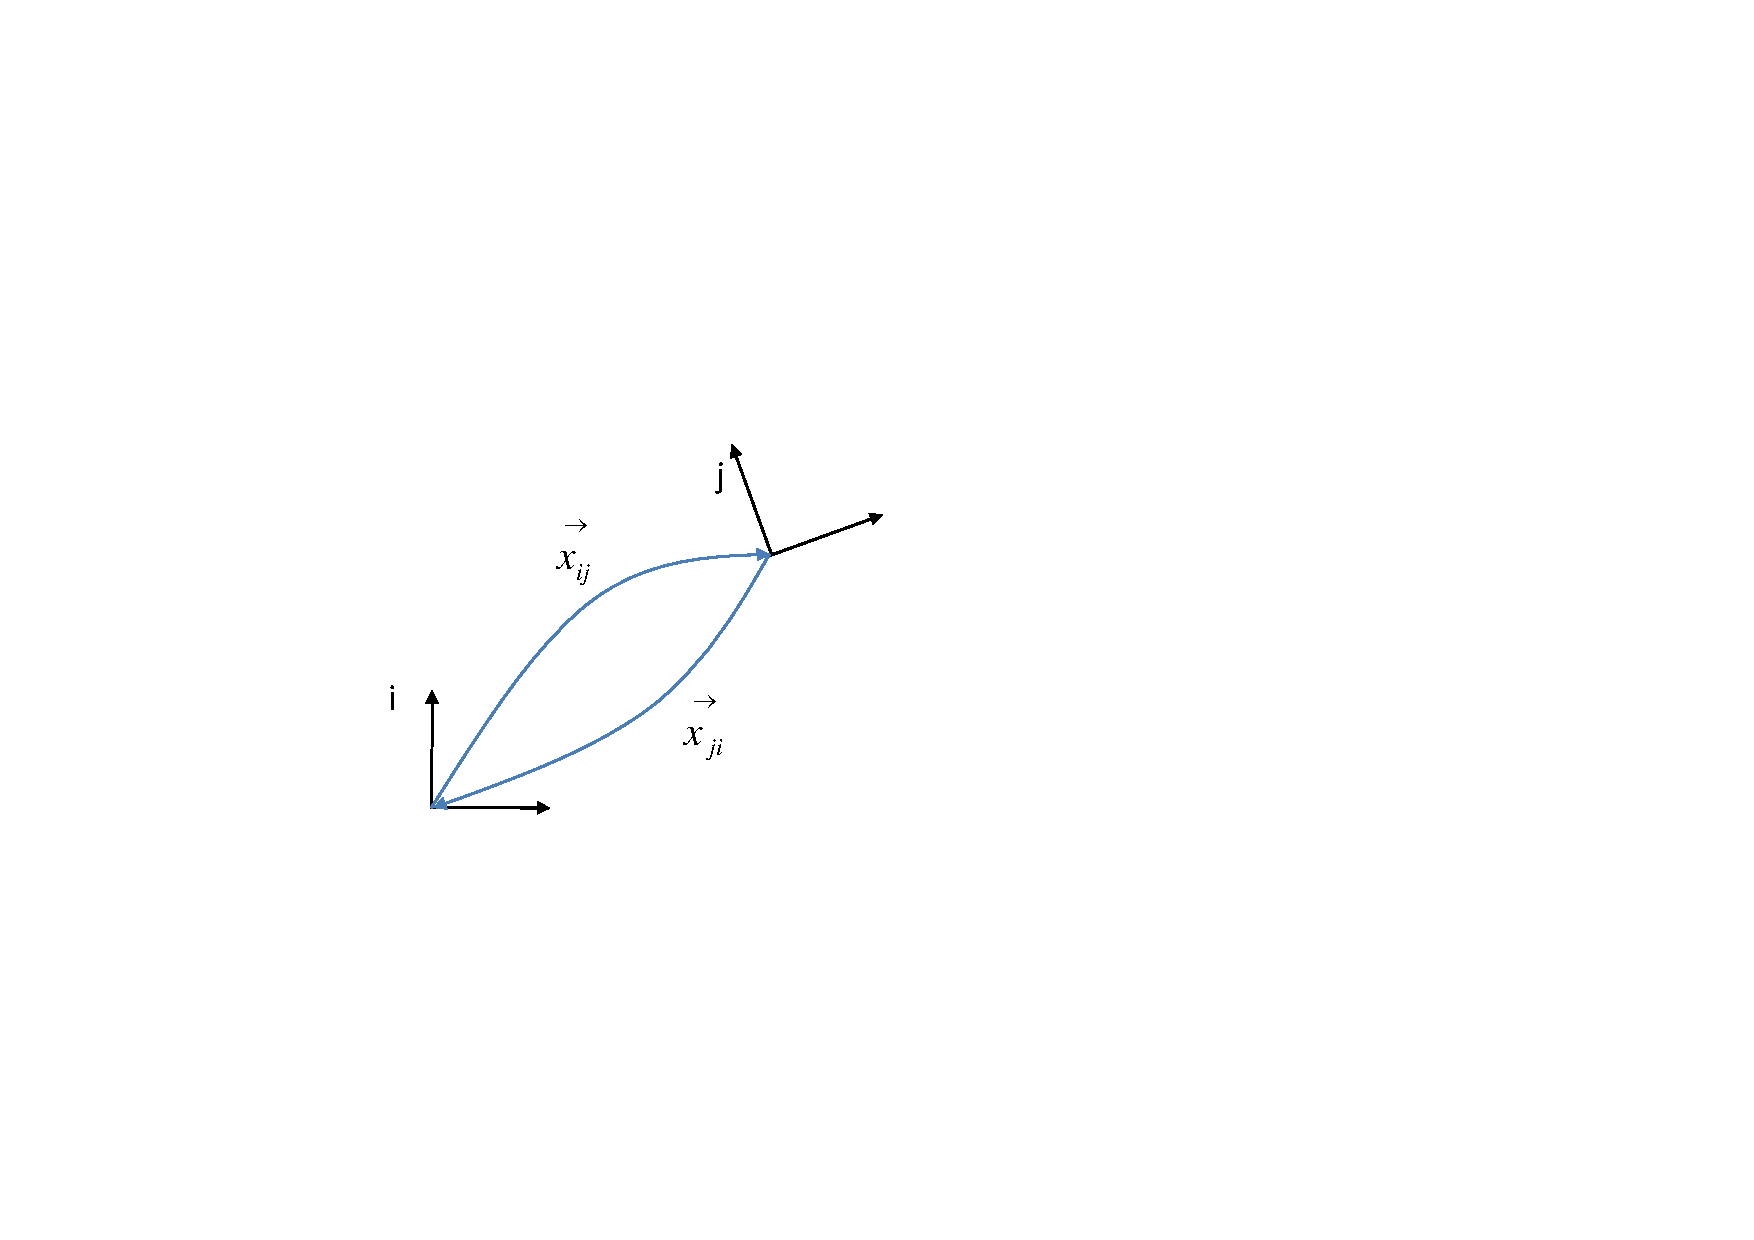
\includegraphics[width=0.5\textwidth]{inv}\\
  \caption{Inversión de una transformación relativa}\label{fg:inv}
\end{figure}

Si $x_{ij}$, $x_{jk}$ y $x_{ik}$ son tres transformaciones relativas tales que $x_{ik} = x_{ij} \oplus x_{jk}$ entonces se verifican las siguientes ecuaciones:

\begin{eqnarray}
% \nonumber to remove numbering (before each equation)
    x_{ik} \neq x_{jk} \oplus x_{ij} \nonumber\\
    x_{ij} = x_{ik} \ominus x_{jk} \nonumber\\
    x_{jk} = \ominus x_{ij} \oplus x_{ik} \nonumber\\
    \ominus x_{ik} = \ominus(x_{ij}\oplus x_{jk}) = \ominus x_{ij} \oplus (\ominus x_{jk})
\end{eqnarray} 